\chapter{Parallel Computing}

The popularity of computational chemistry can be attributed in no small part to the advances and devlopment of highly efficient algorithms in theoretical chemistry. Equally important however is the ever increasing accessibility and performance of computing resources: commercially available work stations can handle chemical systems which could only be modelled on supercomputers a couple decades ago, and firmly cemented the position of computational chemsitry as an important "experimental" tool in the toolbox of a chemist. 

As the speed of computers increased over the years, so did the complexity of their components. Nowadays, programmers can choose between several types of architectures, such as shared or distributed memory systems, or accelerators like GPUs. Knowing the strenths and weaknesses of each type is paramount to developing efficient algorithms and tackling larger molecular systems.

This chapter gives an overview on computer architecture, and the different types of parallelism encountered on modern hardware.

\section{Moore's Law}

\emph{Moore's Law} states that the transistor density in integrated chips doubles every 12 to 24 months. First formulated in 1965 by Gordon More, his prediction has held up fairly well over the years. However, the technology enabling this trend has changed over the years.

Figure ... shows the trends in clock speed, single-thread performance, power consumption and number of logical cores and transistors for microprocessors from 1970 to 2000. Since the early 2000s, clock-speed and single-thread performance have begun to plateau, and have stagnated from 2010 onwards. Increasing the clock speed to values beyond 4 to 5 GHz generates too much stress on the microchip in form of heat, and decreases its performance. This flaw was compensated by using the growing transistor density to instead increase the number of logical cores on a single chip. 

Shifting towards increasing core count however entails that the most ideal perfpormance of a CPU can only be achieved though parallel programming. With the rise of parallel computing, the number of different parallel hardware features drastically increased, and it can be difficult for programmers to fully exploit the available computing resources. Moreover, different programming language and compiler extensions have emerged alongside, with numerous competing standards, especially for GPUs. 

\begin{figure}
\centering
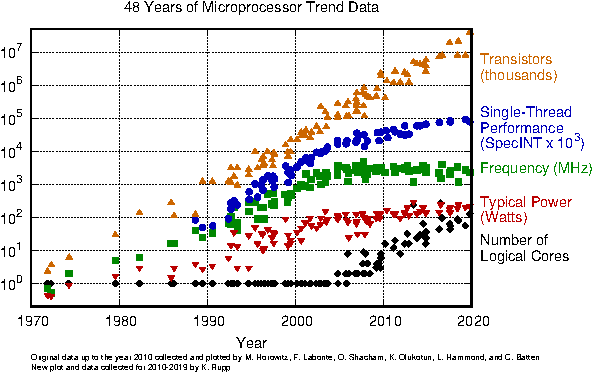
\includegraphics[scale=1.2]{Pics/moore}
\caption{Taken from \protect\url{https://github.com/karlrupp/microprocessor-trend-data}}
\end{figure}

\section{Benefits and Limits of Parallel Computing}

While the different available programming models can seem daunting at first, one of the major advantages of parallel computing is improved \emph{scalabilty}. An application that exposes parallelism can be sped up by several orders of magnitude, simply by adding more compute power, with several different architectures to choose from. The limit of what problem sizes can be tackled is mostly dictated by the \emph{amount} of available computing resources and storage, rather than individual processor charcterstics.

As important as parallel computing has become in recent years, there is a reason why increasing clock speed was seen as the foremost strategy in keeping Moore's law alive. First, modifying a serial program to exploit parallelism can be a time-consuming endeavour, and second, not all tasks can be effectively parallelized. This means that the potential amount of seed-up is limited by the amount of parallel code. This is known as \emph{Amdahl's law}. The speed-up for a number of cores $N_c$ is given by
\begin{equation}
Speed-Up(N_c) = \frac{1}{S + \frac{P}{N_c}}
\end{equation}
\noindent where $S$ is the fraction of serial code and $P$ is the fraction of parallel code. The speedup for a fixed-size problem as a number of cores is known as \emph{strong scaling}, and the time-to-solution on each indivual core \emph{decreases} when more cores are added.

An alternate way to compute potential speed-up is given by Gustafson-Barsis's Law
\begin{equation}
Speed-Up(N_c) = N_c - S(N_c-1)
\end{equation}
\noindent where the problem size also increases proportionally to the number of cores. The scaling for this trend is known as \emph{weak scaling}. In this scenario, the time-to-solution spend on each core remains constant, as the system size and number of cores increases. Even if this type is called "weak", both forms of scaling are equally important, as they adress different scenarios. 

\section{Types of Parallelism and Memory Hierarchy}

Nowadays, a programmer has access to four categories of parallelism:
\begin{enumerate}
\item vectorization
\item thread-based parallelism
\item process-based parallelism
\item streaming
\end{enumerate} 
\noindent Leveraging the power of each type requires some understanding of the underlying hardware. 

Figure \ref{clusterArchitecture} shows the major components and memory pathways in a modern computing cluster. A \emph{cluster} is a collection of individual computers that work together and form a single unit. Individual computers are also called \emph{nodes} and occupy a single rack (or "shelf") each in a large server cabinet. The nodes are connected via a low-latency, high through-put network, e.g. ethernet cables to enable inter-node communication. Each node contains one or more central proecessing units (CPU) and optionally one or more graphical processing units (GPU). Systems where different types of hardware architecture are mixed are also known as \emph{heterogenous} systems. The individual components are fixed on a \emph{motherboard}: CPUs are plugged into \emph{sockets} and GPUs into \emph{PCIe slots}. A CPU is composed of one or more cores, where the actual processing of data is carried out. A GPU is also composed of multiple cores, which are grouped into independent \emph{streaming multiprocessors} (SM). 

\begin{figure}
\centering
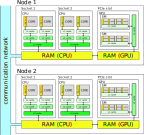
\includegraphics[scale=1.0]{Pics/memory}
\caption{Memory hierarchy}
\label{clusterArchitecture}
\end{figure}

Memory is also a crucial component of computer architecture and is a limited resource. The speed at which data is read from memory can also become a major bottle-neck: No matter how fast a processor is, if the feed rate is too low, it cannot reach its peak performance becuase it wastes cycles while waiting for data to arrive. To optimize data through-put, the memory model in modern computer architecture requires a complex hierarchy, with different sizes and speeds. Computer memory at the top of the hierarchy has a high response rate, but low complexity. It is also very expensive to produce and therefore much smaller. At the bottom of the hierarchy is memory with large storage space and capable of complex tasks. It is cheap but has low reponse rate. Over the years, the number of levels in the memory hierarchy has increased. Most modern computers have six levels: CPU registers, L1 chache, L2 chache, L3 chache, DRAM and disk. 

CPU registers sit at the top of the hierarchy and are closest to the cores. It is the region of memory where data is directly manipulated by arithmetic operations and machine code. Its size is typically on the order of several tens to hundreds of bytes. Data is loaded into the registers from \emph{cache}, a region of memory which is further subdivided into different levels named L1, L2 and L3. Each core has its own L1 cache, but might share L2 and L3 cache with other cores. Caches have different sizes and speeds, with L1 being the fastest and smallest at several tens of kB, and L3 being the slowest and largest at several tens to hundreds of kB. Memory is transferred from L3, to L2, to L1 and finally to the CPU registry. The reason why there are multiple levels of chache is to reduce \emph{cache misses}. If data requested by the core is not found in L1, then L2 is searched, then L3. A cache miss is an event where the data is not found anywhere in chache. In that case, a request has to be put out to the dynamical random access memory (DRAM) to retrive data. Modern techniques such as \emph{chache prefetching} can minimize the amount of cache misses by loading the data into higher chache levels before it is actually needed by the lower levels. 

The speed of DRAM is 10 to 100 time slower than cache, but much larger in size. It is the main memory pool and shared by all cores. CPUs and GPUs have separate DRAM regions which communicate via a PCIe bus. DRAM sizes vary drastically, and are on the order of 10$^0$ to 10$^1$ for GPUs and 10$^0$ to 10$^3$ for CPUs. Data can be transferred from one node to another via CPU DRAM through the communication network, with transfer rates on the order of several GB/s. For programs which are not reading from disk, this is weakest link in the memory hierarchy ???

\section{Vectorization}

Vectorization is the pocess of operating on multiple variables at the same type. This type of parallelism is encountered at the highest level of the memory hierarchy introduced in the previous section, i.e. CPU registers. Each core has multiple registers, also called \emph{vector registers} with a certain size or \emph{vector length}. Instead of loading each inidividual element from cache and operating on it, one vector operation on a range of elements can replace multiple single operations. For a 512-bit register, two vectors with 8 floats (32 bit) can be summed within one cycle instead of eight (Figure ...). This type of parallelism is also known as single instruction multiple data (SIMD). 

The length of vector registers, number of registers as well as the number of supported vector operations have greatly expanded over the years (Table \ref{VECTORHARDWARE}).

\begin{table}
\makegapedcells
\centering
\begin{tabular}{p{0.3\linewidth}cc}
\hline
Release & Vector Length (bit) & No. Registers \\ \hline
SSE (Streaming SIMD Extension) & 128 & 8 \\ 
SSE2/SSE3/SSE4 & 128 & 16  \\
AVX/AVX2 (advanced vector instructions) & 256 & 16 \\
AVX512 & 512 & 32 \\ 
\hline 
\end{tabular}
\caption{Adpated from ...}
\label{VECTORHARDWARE}
\end{table}

\subsection{Parallel SAXPY using vectorization}

To show how vectorization can be introduced into a program, consider the following vector operation:
\begin{equation}
y \leftarrow \alpha x + y
\label{DAXPY}
\end{equation}
\noindent where $y$, $x$ are vectors of equal length, and $\alpha$ is a scaling factor. The vector operation \ref{DAXPY} is also known as "saxpy" for single precision, and "daxpy" for double precision. A naive implementation of the saxpy-kernel is given in Listing \ref{lst:SAXPYNOPARA} for vector size $N$  

\cppcode{Parallelization-unaware implementation of saxpy \label{lst:SAXPYNOPARA}}{saxpy_nopara.c}

\noindent Two arrays are allocated, x and y, and all their entries set to 1 and 2 respectively. Each element is updated individually in the for loop. There are several possibilities to introduce vectorization:
\begin{enumerate}
\item auto-vectorization
\item compiler directives
\item intrinsic functions
\item optimized libraries
\end{enumerate}
\noindent Auto-vectorization is by far the easiest approach: the compiler automatically recognizes that the loop can be vectorized and generates optimized machine code that uses vector instructions. This does not require any input from the user. Compiling the code on a machine with AVX support, using the GNU C compiler, and passing the compiler flags "-O2 -march=native -ftree-vectorize -fopt-info-vec-optimized" generates the following report:
\begin{lstlisting}[backgroundcolor=\color{light-gray},breaklines=true]
saxpy_nopara.c:9:3: optimized: loop vectorized using 32 byte vectors
\end{lstlisting}
\noindent which indicates that the vectors are loaded and operated on in 32 byte chunks, or 8 floats at once. The flag "-ftree-vectorize" (or alternatively "-O3") activates auto-vectorization and "-fopt-info-vec" generates the report. To make sure that the C compiler uses the right vectorization relase, the flag "-march=native" is needed, or else the comiler might fall back to SSE. 

In some cases, auto-vectorization cannot take place because the compiler did not recognize that the loop can be vectorized. It can then be beneficial to use \emph{intrinsic functions}. Intrinsic functions are compiler-dependent functions that map to processor operations. When targeting an AVX architecture with 256-bit registers, the saxpy kernel can be rewritten as
\cppcode{SAXPY using intrinsics \label{lst:SAXPYINTRINSICS}}{saxpy_intrinsic.c}
\noindent It is apparent that using intrinsics makes the program much more complex. The arrays cannot be fed directly to the functions, but need to be loaded into vectors of type \texttt{\_\_mm256}, using "set" or "load" functions. Furthermore, the data needs to be aligned correctly using \texttt{\_\_attribute\_\_ ((aligned(...)))}. The arrays are then loaded in chunks into the registers and given to the vector functions for multiplying and adding. 

The major problem with using intrinsic functions, besides increased complexity, is \emph{portability}. The code in \ref{lst:SAXPYINTRINSICS} does not compile on machines that do not support AVX, and is limited to 256-bit registers even on AVX-512 machines. Portable alternatives include using compiler directives or optimized libraries.

Directives (or "pragmas") are hints that can be given to the compiler that suggest that the loop might be vectorizeable. By far the most popular set of compiler directives that provide vectorization capabilities is undoubtedly included in the OpenMP application programming interface (API). The OpenMP API is standardized accross all compilers, making it highly portable. The OpenMP directives greatly simplify the SAXPY program:
\cppcode{SAXPY using compiler directives \label{lst:SAXPYDIRECTIVES}}{saxpy_openmp.c}
\noindent Simply plopping the directive in front of the for loop takes care of generating the appropriate machine code for the targeted architecture. 

The last way to introduce vectorization is via external programs, such as the basic linear algebra subprograms (BLAS) library. It provides a set of specific functions for performing basic vector and matrix operations. Similar to OpenMP, it only provides spcifications, and the direct implementation is compiler-dependent. In the BLAS routines, there is a saxpy functions available that can be called directly. It has the advantage of completely removing the loop and clearly states what operation is performed.
\cppcode{SAXPY using BLAS \label{lst:SAXPYBLAS}}{saxpy_blas.c}
\noindent External libraries can however be associated with a steeper learning curve depending on the complexity of function signatures.

\section{Thread-based Parallelism}

\section{Process-based Parallelism}

\section{Steaming}

Why parallel computing?
-> becomes increasingly important, programmers should be well versed in it

Moores's Law

Fundamental law's: Amdahl

Types of parallelism:
- vectorization
- threads
- processes
- streaming (GPU)

Work at different levels of hardware

SETI@HOME

Categorizing parallel approaches Flynn's Taxonomy

errors in parallelism (p.40-41)

Performance limits
Levels of memory : speed vs feed (p. 59) show example of sizes of L caches

